\documentclass{jarticle}
\usepackage[dvipdfmx]{graphicx}
\usepackage{here}
\usepackage{listings,jlisting}
\usepackage{amsmath}

\lstset{
  basicstyle={\ttfamily},
  identifierstyle={\small},
  commentstyle={\smallitshape},
  keywordstyle={\small\bfseries},
  ndkeywordstyle={\small},
  stringstyle={\small\ttfamily},
  frame={tb},
  breaklines=true,
  columns=[l]{fullflexible},
  numbers=left,
  xrightmargin=0zw,
  xleftmargin=3zw,
  numberstyle={\scriptsize},
  stepnumber=1,
  numbersep=1zw,
  lineskip=-0.5ex
}

\title{{$B%7%9%F%`<B83(B}\\$B<B838e4|Bh(B4$B2s%l%]!<%H(B}
\author{6119019056 $B;38}NOLi(B}
\date{2019/10/31$BF|Ds=P(B}
\begin{document}
\maketitle
\section{$B%l%]!<%H(B11.4.1}
$B2]Bj(B11.4.1($B4pK\F0:n$N3NG'(B)$B$G$O(B,$B%+%i!<%;%s%5!<$N%-%c%j%V%l!<%7%g%s$r9T$J$C$F$$$k(B.$B6qBNE*$K$I$N$h$&$J%-%c%j%V%l!<%7%g%s$r9T$J$C$F$$$k$+(B,$B%W%m%0%i%`$NCf?H$rFI$s$G@bL@$;$h(B. \\

$B%;%s%5!<$,CM$rFI$_9~$`$?$S$K$=$l$>$l(Bred,green,blue$B$N%;%s%5!<$NCM$rB-$7$F9T$-(B,$B$=$l$r%+%&%s%H$G3d$C$F9T$/(B.$B%+%&%s%H$b%;%s%5!<$NCM$rFI$_9~$`$?$S$KA}$($F9T$/$?$a%+%i!<%;%s%5$NFI$_<h$C$?CM$NJ?6QCM$rD4$Y$F$$$k$3$H$K$J$k(B.

\section{$B%l%]!<%H(B11.4.2}
$B2]Bj(B11.4.2(bang-bang$B@)8f$K$h$k%i%$%s%H%l!<%9(B)$B$K$*$$$F(B,$K_p$$B$NCM$N0c$$$K$h$C$F%i%$%s%H%l!<%9$,$I$N$h$&$KJQ2=$7$?$+5-=R$;$h(B.$B$^$?(B,bang-bang$B@)8f$NLdBjE@$r@bL@$;$h(B. \\

$K_p$$B$NCM$rA}$d$9$H(Bzumo$B$N:81&$KF0$/I}$,9-$,$j$h$j<X9T$9$k$h$&$K$J$C$?(B.$K_p$$B$NCM$r>.$5$/$9$k$H(Bzumo$B$N:81&$KF0$/I}$O>.$5$/$J$C$?$,(B,$B5^%+!<%V$J$I$O6J$,$l$J$/$J$C$?(B. \\
bang-bang$B@)8f$G$OL\I8CM$KBP$7$F>o$K0lDj$NG\N((B($K_p$)$B$G$7$+B.EY$r@)8f$G$-$J$$$N$G(B,$BL\I8CM$rD6$($k$+L\I8CM$r2<2s$k$+$G$D$M$K?6F0$7$F$7$^$&$N$,LdBjE@$G$"$k(B.

\section{$B%l%]!<%H(B11.4.3}
$B2]Bj(B11-4.3(P$B@)8f$K$h$k%i%$%s%H%l!<%9(B)$B$K4X$7(B,$B2<5-(B(a)~(d)$B$4$H$KJ,$1$F%l%]!<%H$r:n@.$;$h(B.
(a)$B:n@.$7$?%W%m%0%i%`$rJs9p$;$h(B.
(b)bang-bang$B@)8f$H(BP$B@)8f$N>l9g$G%i%$%s%H%l!<%9$NF0:n$,$I$N$h$&$K0c$C$?$+5-=R$7(B,$B$J$<$=$N$h$&$K$J$k$N$+86M}$r@bL@$;$h(B.(c)$K_p$$B$NCM$N0c$$$K$h$C$F%i%$%s%H%l!<%9$,$I$N$h$&$KJQ2=$7$?$+5-=R$;$h(B.(d)$B9bB.$+$D%9%`!<%:$K%i%$%s%H%l!<%9$r9T$&$3$H$,$G$-$?(B$K_p$$B$NCM$H(Bspeed$B$NCM$rJs9p$;$h(B.$B$^$?(B,$B@V(B,$BNP(B,$BNP(B,$B@V$N6h4V$rDL2a$7$?:]$N(BRGB$B$NCM$NJQ2=$N%0%i%U$rE=$jIU$1(B,$B$I$N$h$&$JFCD'$,$"$k$+9M;!$;$h(B.

\subsection{(a)}
$B0J2<%=!<%9%3!<%I(B\ref{code:kadai3}$B$K:n@.$7$?%W%m%0%i%`$rJs9p$9$k(B.

\begin{lstlisting}[caption = P$B@)8f(B,label=code:kadai3]
if ( lightNow < (lightMin + lightMax) / 2.0 ) // $B1&2sE>(B
    //P$B@)8f(B,lightNow$B$NCM$K1~$8$F(BspeedDiff$B$NCM$r@~7A$KJQ2=(B
    speedDiff = map(lightNow,lightMin,(lightMin+lightMax) / 2.0, -Kp*speed,0);
else // $B:82sE>(B
//P$B@)8f(B,lightNow$B$NCM$K1~$8$F(BspeedDiff$B$NCM$r@~7A$KJQ2=(B
  speedDiff = map(lightNow,(lightMin+lightMax) / 2.0,lightMax,0,Kp*speed);
  motorL_G = speed - speedDiff;
  motorR_G = speed + speedDiff;
\end{lstlisting}

\subsection{(b)}
bang-bang$B@)8f$G$OL\I8CM$KBP$7$F?6F0$7$F$$$?$,(B,P$B@)8f$G$OL\I8CM$K6a$1$l$P6a$$$[$IA`:nNL$r8:$i$9$?$a(B,$BD>@~$G$bL\I8CM$K6a$E$/$H?6F0$;$:$K0lDj$NF0$-$r$7$F$$$?(B.
\subsection{(c)}
$K_p$$B$NCM$,Bg$-$/$J$k$H5^%+!<%V$K$OBP1~$G$-$k$h$&$K$J$C$?$,(B,$B>/$7(Bbang-bang$B@)8f$K6a$$$h$&$JF0$-$K$J$C$?(B.$K_p$$B$NCM$,>.$5$$$H%9%`!<%:$G$O$"$k$,5^%+!<%V$J$I$OBP1~$G$-$J$+$C$?(B.

\subsection{(d)}
$B9bB.$+$D%9%`!<%:$K%i%$%s%H%l!<%9$G$-$?CM$O$=$l$>$l(B$K_p$ = 1.9,speed=100$B$G$"$C$?(B.
$B$^$?(B,$B0J2<?^(B\ref{fig:chokusen},$B?^(B\ref{fig:kyokusen}$B$KD>@~$H6J@~$N>l9g$N?^$r<($9(B.
\begin{figure}[H]
\begin{center}
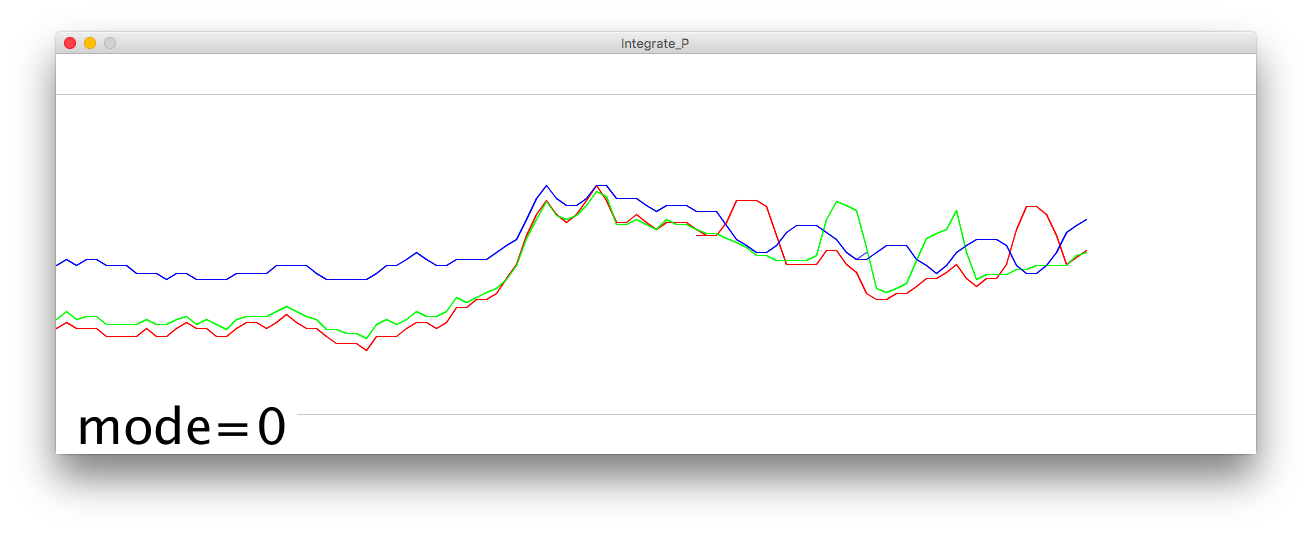
\includegraphics[width=7.0cm]{images/chokusen.png} 
\caption{$BD>@~$N>l9g(B}
\label{fig:chokusen} 
\end{center} 
\end{figure} 

\begin{figure}[H]
\begin{center}
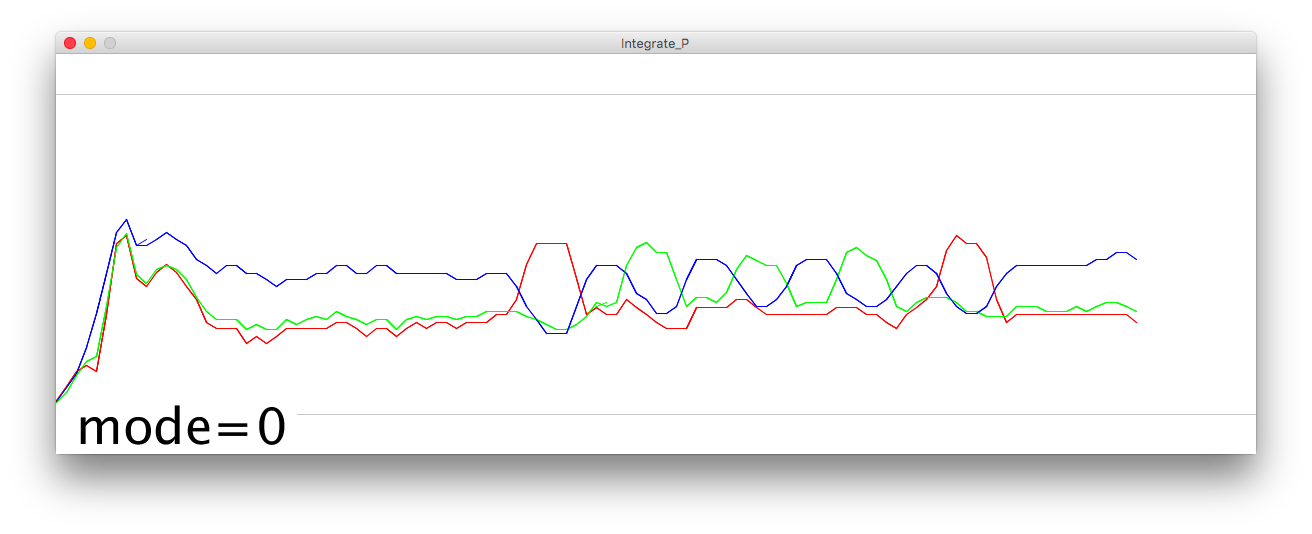
\includegraphics[width=7.0cm]{images/kyokusen.png} 
\caption{$B6J@~$N>l9g(B}
\label{fig:kyokusen} 
\end{center} 
\end{figure} 
$B6J@~$NJ}$,A4BNE*$J(BRGB$BCM$,D>@~$KHf$Y$FDc$+$C$?(B.
\section{$B%l%]!<%H(B11.4.4}
$B2]Bj(B11-4.4$B$G$O(Bloop$B4X?t$r@)8f$N4pK\C10L$H$7$?%W%m%0%i%_%s%0J}?K$r3X$s$@(B.$B$3$N%W%m%0%i%`J}?K$NNXE>$r5-=R$;$h(B.\\
mode$B$K$h$C$F>uBV$rA+0\$9$k$N$GB>$N5-=RItJ,$O8+$J$/$F$h$$$N$G(B1$B2s$N(Bloop$B$K$+$+$k<B9TB.EY$,C;$/$J$k(B.$B$^$?(B,$B%3!<%I$bFI$_$d$9$/$o$+$j$d$9$$(B.

\section{$B%l%]!<%H(B11.4.5}
$B2]Bj(B11-4-5$B$G:n@.$7$?%W%m%0%i%`$rJs9p$;$h(B.$B$^$?(B,$B$I$N$h$&$J>uBVA+0\$r9T$J$C$?$+@bL@$;$h(B. \\

$B0J2<%=!<%9%3!<%I(B\ref{code:kadai5}$B$K:n@.$7$?%W%m%0%i%`$rJs9p$9$k(B.

\begin{lstlisting}[caption = $B2]Bj(B11-4.5,label=code:kadai5]
switch ( mode_G ) {
   case 0:
     mode_G = 1;
     break;  // break$BJ8$rK:$l$J$$!JK:$l$k$H$=$N2<$b<B9T$5$l$k!K(B

   case 1:
     linetrace_P(); // $B%i%$%s%H%l!<%9!J3F<+$G:n@.!K(B
     color = identify_RGB(); // $B%i%$%s$N?'$r?dDj(B(R:$B@V!$(BG:$BNP!$(BB:$B@D!$(B-:$B$=$l0J30!K(B
     if ( color == 'R' ) { // red //$B0l2sL\$N@V(B
         mode_G = 2;
        }
     break;
   case 2:
     linetrace_P();
     color = identify_RGB();
     if( color == 'B' ) {
       mode_G = 3;  
	  }
     break;
   case 3: 
     linetrace_P(); // $B%i%$%s%H%l!<%9(B
     color = identify_RGB();
     if ( color == 'R' ) { //$B#22sL\$b@V$@$C$?$i(B
      startTime = timeNow_G; // mode_G=3$B$KA+0\$7$?;~9o$r5-O?(B
      mode_G = 4;
      }
     if ( color == 'G' ) { //2$B2sL\$,NP$@$C$?$i(B
         green_count++;
         mode_G = 5;
     }
     break;
    
   case 4:
     motorL_G = 100;
     motorR_G = 100;
     if ( timeNow_G - startTime > run_period ) // $B;XDj;~4V7P2a$7$?$i(B
      mode_G = 1;
     break;
   case 5:
     linetrace_P();
     color = identify_RGB();
     if (color == 'B') {
       mode_G = 6;
     }
     break;
   case 6:
     linetrace_P();
     color = identify_RGB();
     if( color  == 'G') { //$BNP$@$C$?$i%+%&%s%H(B
       green_count++;
       mode_G=5;
     }
     if ( color == 'R') { //$B@V$@$C$?$i=*N;(B
       motorL_G = -100;
       motorR_G = 100;
       delay(500);
       mode_G = 7;
     }
     break;
   case 7:
     color = identify_RGB();
     motors.setSpeeds(100,100);
     if( color == 'B') {
       mode_G = 8;
      }
      break;
    case 8:
      color = identify_RGB();
      motors.setSpeeds(100,100);
      if( color == 'W') {
        mode_G = 9;
      }
      break;
    case 9:
      delay(1000);
      for(int i = 0; i < green_count; i++) {
        motors.setSpeeds(100, 100); // $BD>?J(B
        delay(500);
        motors.setSpeeds(0, 0); // $BDd;_(B
        delay(500);
      }
      mode_G = 10;
      break;
    case 10:
      motors.setSpeeds(0,0);
      break;
}

\end{lstlisting}
$B$^$?(B,$B0J2<?^(B\ref{fig:kadai5}$B$K%U%m!<%A%c!<%H?^$r<($9(B.
\begin{figure}[H]
\begin{center}
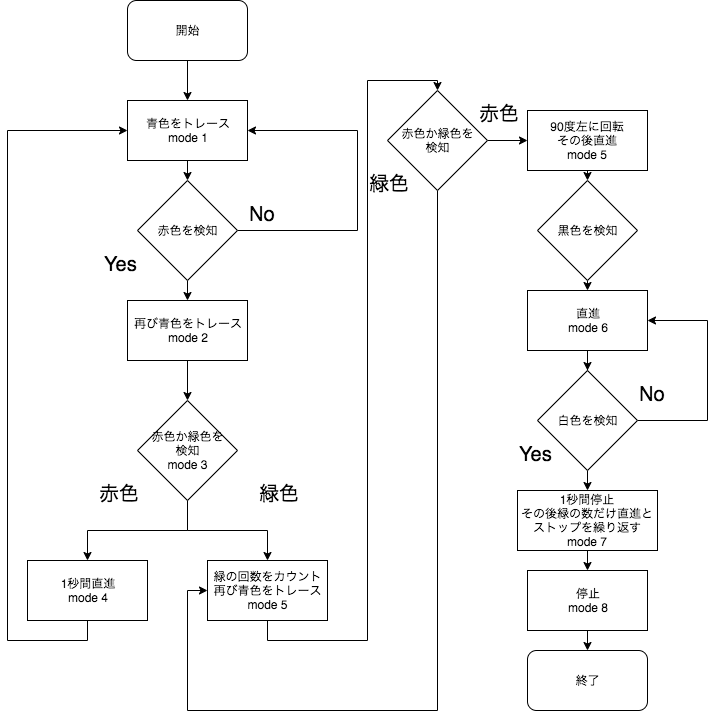
\includegraphics[width=9.0cm]{images/kadai5.png} 
\caption{$B%U%m!<%A%c!<%H?^(B}
\label{fig:kadai5} 
\end{center} 
\end{figure} 


\end{document}
